\documentclass[landscape,twocolumn]{article}
\usepackage{biblatex, pgfplots, pgfplotstable}
\usepackage{biblatex, graphicx, pgfplots, pgfplotstable}
\addbibresource{references.bib}
\pgfplotsset{compat = 1.16}
\title{COMP5318 Assignment 1}
\author{Nicholas Grasevski (ngra5777, 500710654)}
\begin{document}
\maketitle
\begin{abstract}
In this report several image classifiers are benchmarked against a grayscale image dataset. With the help of some feature engineering, a linear Support Vector Machine is the highest performing classifier with 89.65\% accuracy on the test set.
\end{abstract}

\section{Introduction}
\begin{itemize}
\item What is the aim of the study?
\item Why is the study important?
\end{itemize}

\begin{figure}[ht]
\caption{Grayscale 28x28 images of clothing.}
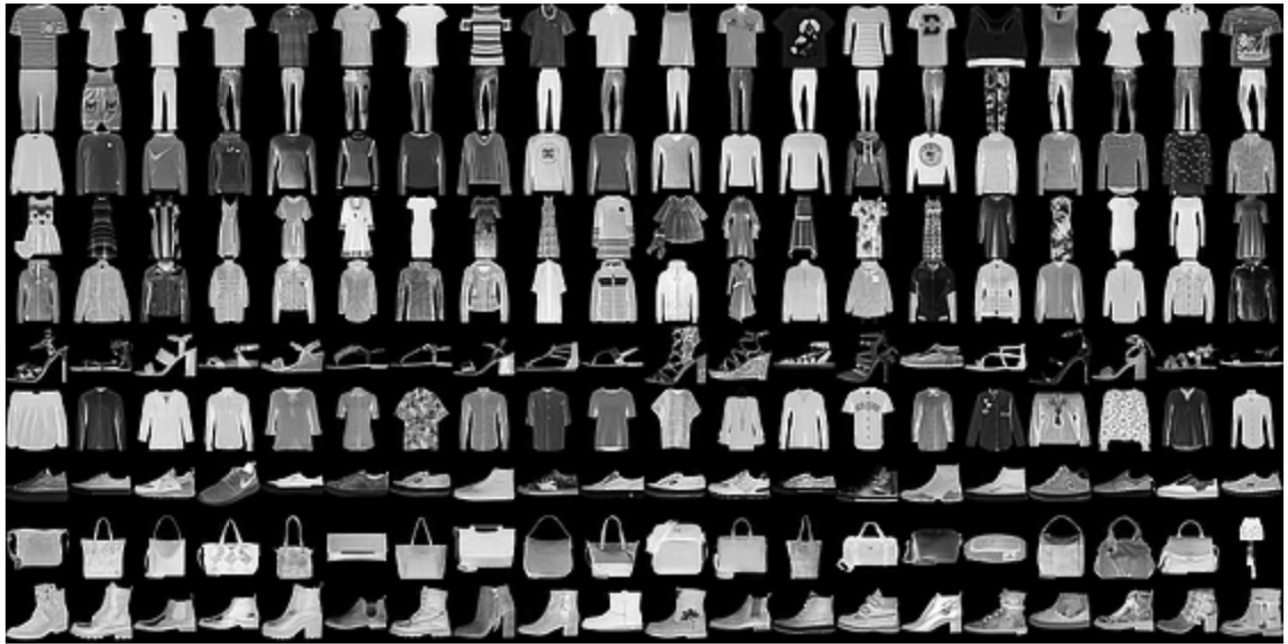
\includegraphics[width=\linewidth]{../Dataset_image}
\end{figure}

\section{Methods}
Describe the pre-processing techniques and classifier methods algorithms.

\section{Experiments and results}
Comparing experiment results between different algorithms (using table or graph) and produce a meaningful discussion of results from the experiment and choice of classifier methods (analysis on potential reasons for good performance or bad performance, and for training and inference time consumption).

\section{Conclusion}
Meaningful conclusion based on results, future work, and improvement suggested.

\printbibliography\appendix
\section{Running the code}
\begin{itemize}
\item Dependencies: \texttt{pip3 install h5py pandas scikit-image scikit-learn}
\item Usage: run the steps in the notebook sequentially to get the tuning and evaluation results.
\end{itemize}
Detailed hyperparameter tuning results will be written as csv files to \texttt{Algorithm/Output} for each respective classifier, along with the final predictions as \texttt{Algorithm/Output/predicted\_labels.h5}.

\end{document}
